\documentclass[a4paper, 12pt]{article}
\usepackage[a4paper, top = 1.5cm, bottom = 1.5cm, left = 1cm, right = 1cm]{geometry}
\usepackage[english, russian]{babel}
\usepackage{graphicx}
\usepackage{subcaption}
\usepackage{mathtools}
\usepackage{amsfonts}
\usepackage{float}
\title{Лабораторная работа № 4.8А "Резонанс токов"}
\author{Кирилл Шевцов Б03-402}
\date{16.10.2025}
\begin{document}
\maketitle
\section*{Лабораторная установка}
\begin{figure}[htbp]
    \centering
    \includegraphics[width=0.7\linewidth]{equip.png}
    \label{Лабораторная установка}
    \caption{Лабораторная установка}
\end{figure}
Задание предполагает снятие зависимости значений тока на учасках с амперметрами от индуктивности катушки.
Согласно установке : амперметр $A_{1}$ показывает общий ток в цепи, $A_{2}$ - ток на участке с катушкой, $A_{3}$ - ток на конденсаторе заданной
заданной емкости $C = 120$ мкФ.\newline Напряжение подается от сети постоянным $U = 220$ В, частота генератора также постоянна и равна $\nu = 50$ Гц.\newline
Картину резонанса можно увидеть либо по минимальному току на амперметре $A_{1}$, либо на осциллорафе: резонансу соответсвует нулевой сдвиг фазы,
то есть вырождение эллипса в наклонную прямую.\newline
Резонанс токов полагается исследовать на параллельном колебательном контуре, поскольку напряжение на участках цепи, параллельных включенному
вольтметру, совпадают.
\section*{Измерения и результаты}
\begin{enumerate}
    \item Будем медленно вдвигать сердечник в катушку индуктивности. Зафиксировав расстояние, на которое вдвинут сердечник, снимем показания
    амперметров $A_{1}$, $A_{2}$, $A_{3}$. Ток на учатках с катушкой, кондесатором и общий ток обозначим соответсвенно $I_{L}$, $I_{C}$, $I$.
    \begin{table}[htbp]
        \centering
        \begin{tabular}{|c|c|c|c|c|c|c|c|c|c|c|c|}
            \hline
            $x$, см & 7.0 & 6.5 & 6.0 & 5.5 & 5.0 & 4.5 & 4.0 & 3.5 & 3.0 & 2.5 \\
            $I_{L}$, А & 0.417 & 0.387 & 0.354 & 0.325 & 0.301 & 0.277 & 0.255 & 0.233 & 0.213 & 0.186 \\
            $I_{C}$, А & 0.401 & 0.395 & 0.392 & 0.393 & 0.386 & 0.398 & 0.395 & 0.395 & 0.398 & 0.391 \\
            $I$, А & 0.05 & 0.045 & 0.056 & 0.078 & 0.100 & 0.125 & 0.144 & 0.164 & 0.186 & 0.207 \\
            \hline
        \end{tabular}
        \caption{снятие токов при вдвижении сердечника}
        \label{снятие токов при вдвижении сердечника}
    \end{table}\newline
    Обозначим четкий диапазон перемещения дросселя $\Delta = 1.5 \div 6.9$ см.
    Напряжение на ЛАТР поддерживаем постоянным и равным $U_{0} = 10.0 \pm 0.1$ В.
    Частота лабораторного трансформатора $\omega = 50\pm 1$ Гц.
    Емкость конденсатора $C = 120\pm 10$ мкФ.
    \newpage
    \item Построим графики зависимостей сил тока на рассмотренных участках от положения $x$ сердечника.
    (по горизонтальной оси - расстояние, на которое сердечник выдвинут из катушки)
    \begin{figure}[htbp]
        \centering
        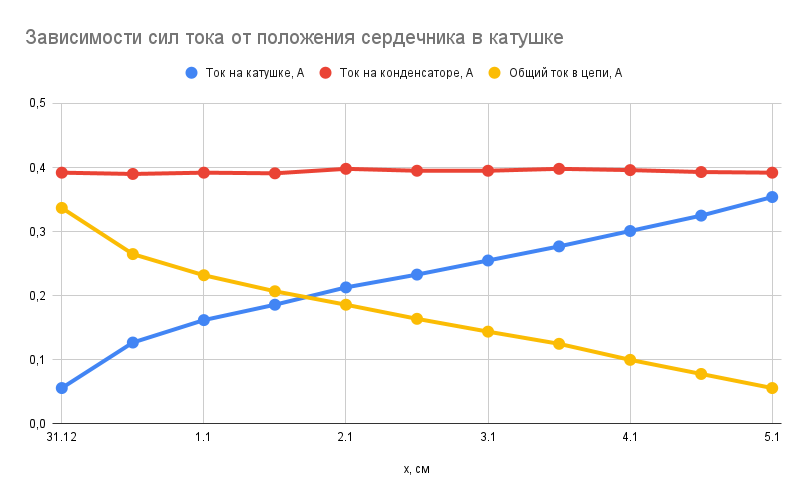
\includegraphics[width=0.6\linewidth]{I_x.png}
        \label{зависимость сил тока для разных расстояний}
        \caption{зависимость силы тока от положения сердечника в катушке}
    \end{figure}\newline
    Из результатов измерений видно, что сила тока на учатке с катушкой постоянно увеличивается, общий ток в цепи уменьшается. Сила тока 
    на участке с конденсатором остается постоянной, поскольку она зависит только от частоты и напряжения генератора.
    \begin{equation}
        I_{C} = U_{0} \omega C = 2\pi \nu C U_{0} = 0.37\pm 0.01\ \text{A}
        \label{ток на участке с конденсатором}
    \end{equation}
    И последние два определяются соотношением
    \begin{align}
        I_{L} = I(L) &= \frac{U_{0}}{\sqrt{(R + r_{L})^{2} + (\omega_{0}L)^{2}}}\\
        I &= I_{L} + I_{C}
    \end{align}
    \item Найдем положение резонанса с помощью осциллографа, запишем резонансные значения тока на рассматриваемых участках цепи.
    \begin{table}[htbp]
        \centering
        \begin{tabular}{|c|c|c|c|c|c|}
            \hline
            $I^{res}_{L}$, А & $I^{res}_{C}$, А & $I^{res}$, А & $\Delta I^{res}_{L}$, А & $\Delta I^{res}_{C}$, А & $\Delta I^{res}$, А\\
            \hline
            0.428 & 0.419 & 0.049 & \multicolumn{3}{|c|}{0.001}\\
            \hline
        \end{tabular}
        \caption{резонансные токи на катушке, конденсаторе и в цепи}
        \label{резонансные токи на катушке, конденсаторе и в цепи}
    \end{table}
    \item Рассчитаем добротность колебательного контура - через токи, и резонансное сопротивление - через полный ток и напряжение.
    \begin{align}
        Q &= \frac{I^{res}_{C}}{I^{res}} = \frac{0.428}{0.049} = 8.55 \pm 0.19, \quad \Delta Q = Q\left(\frac{\Delta I^{res}_{C}}{I^{res}_{C}} + \frac{\Delta I^{res}}{I^{res}}\right) = 0.19\\
        R_{\Sigma} &= \frac{U_{0}}{I^{res}} = \frac{10.00}{0.049} = 204.08 \pm 4.37\ \text{Ом}, \quad \Delta R_{\Sigma} = R_{\Sigma}\left(\frac{\Delta U_{0}}{U_{0}} + \frac{\Delta I^{res}}{I^{res}}\right) = 4.37\ \text{Ом}
    \end{align}
    \item Рассчитаем индуктивность катушки $L_{res}$ через емкость и частоты $\nu = 50$ Гц и $\nu = 50$ Гц, а затем через добротность и емкость сделаем рассчет активного
    сопротивления катушки.(в выражение для частоты учли множитель).
    \begin{align}
        L_{res} = \frac{1}{\omega^{2}C} = 0.084\pm 0.010\ \text{Гн}, \quad
        \Delta L_{res} = L_{res}\left(\frac{2\Delta \omega}{\omega} + \frac{\Delta C}{C}\right) = 0.010\ \text{Гн}\\
        r_L = \frac{\omega L_{res}}{Q} = 3.09\pm 0.49\ \text{Ом},\quad
        \Delta r_L = r_L\left(\frac{\Delta L_{res}}{2L_{res}} + \frac{\Delta C}{C} - \frac{\Delta Q}{Q}\right) = 0.49\ \text{Ом}
    \end{align}
    Расчет для частоты $\nu = 1000$ Гц.
    \begin{align}
        L_{res} = \frac{1}{\omega^{2}C} = 0.021\pm 0.006\ \text{Гн}, \quad
        \Delta L_{res} = L_{res}\left(\frac{2\Delta \omega}{\omega} + \frac{\Delta C}{C}\right) = 0.006\ \text{Гн}\\
        r_L = \frac{\omega L_{res}}{Q} = 15.43\pm 2.49\ \text{Ом},\quad
        \Delta r_L = r_L\left(\frac{\Delta L_{res}}{2L_{res}} + \frac{\Delta C}{C} - \frac{\Delta Q}{Q}\right) = 2.49\ \text{Ом}
    \end{align}
    \item Сравним полученные значения сопротивления и индуктивности со значениями, снятыми с моста $E7-8$ при частоте $\nu = 50$ и $\nu = 1000$ Гц.
    \begin{table}[htbp]
        \centering
        \begin{tabular}{|c|c|c|c|c|c}
            \hline
            Частота, Гц & \multicolumn{2}{|c|}{Расчет с E7-8} & \multicolumn{2}{|c|}{Расчет с графиками}\\
            \hline
            $\nu$, Гц & $L_{res}$, мГн & $r_{L}$, Ом &  $L_{res}$, мГн & $r_{L}$, Ом\\
            $50$ & $67.011\pm 0.001$ & $1.937\pm 0.001$ & $84.00\pm 0.10$ & $3.09\pm 0.49$\\
            \hline
            $1000$ & $60.610\pm 0.001$ & $31.850\pm 0.001$ & $21.000\pm 0.006$ & $15.43\pm 2.49$\\
            \hline
        \end{tabular}
        \caption{Сравнение с полученными данными}
        \label{Сравнение с полученными данными}
    \end{table}\\
    Как видно, измерения сопротивлений снятыми с моста $E7-8$ при частоте $\nu = 50$ отличаются чуть меньше, чем в 2 раза, измерение индуктивности отличаются примерно на 20 мГн.
    Измерения сопротивления для частоты кГц отличаются также в 2 раза, индуктивность отличается почти в 3 раза.
    \item Построим векторные диаграммы резонансных значений тока.
    \begin{figure}[htbp]
        \centering
        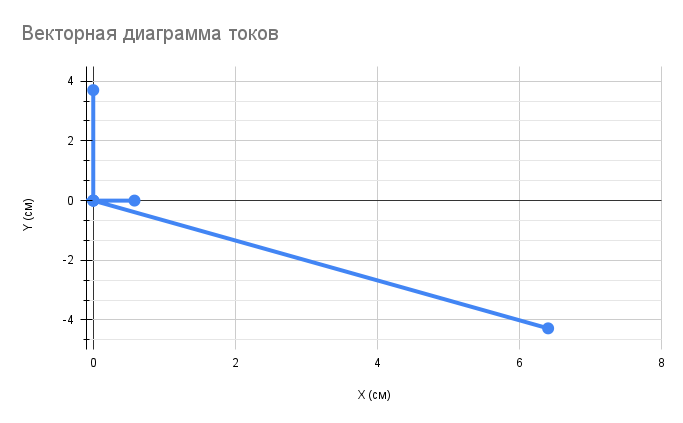
\includegraphics[width=0.7\linewidth]{vec_diag.png}
        \label{треугольная векторная диаграмма}
        \caption{Векторная диаграмма для резонансных токов}
    \end{figure}
    \begin{table}[htbp]
        \centering
        \begin{tabular}{|c|c|c|c|c|c|c|}
            \hline
            & $I_{C}$ нач & $I_{C}$ кон & $I_{L}$ нач & $I_{L}$ кон & $I$ нач & $I$ кон \\
            \hline
            $X$, см & 0 & 0 & 0 & 3.7 & 0 & 0.58 \\
            $Y$, см & 0 & 3.70 & 0 & -4.28 & 0 & 0 \\
            \hline
        \end{tabular}
        \caption{Таблица для векторной диаграммы (масштаб: 0.1)}
        \label{Таблица для векторной диаграммы (масштаб: 0.1)}
    \end{table}\\
    Из графиков видно, что вектор тока на конденсаторе направлен вертикально, ток на катушке смотрит против вертикальной оси, а их сумма
    почти направлена вдоль горизонтальной оси. На первой диаграмме виден "хвостик" графика для координаты $x$ - это активное сопротивление катушки,
    которое присутствует в реальных условиях измерений. Если считать элементы идеальными, то токи $I_{L}$ и $I_{C}$ будут совпадать по величине, то есть компенсировать друг друга.
    \item Построим вектор диаграмму напряжений, напряжение $U_{C}$ считаем постоянным, и равным $U_{0}$.
    На масштаб $S$ делим (то есть умножаем на 10).
    \begin{figure}[H]
        \centering
        \includegraphics[width=0.7\linewidth]{volt_diag.png}
        \label{Векторная диаграмма токов и напряжений}
        \caption{Векторная диаграмма токов и напряжений}
    \end{figure}
    \subsection*{Угол между напряжением и током катушки}
    \begin{align*}
        \sin \varphi = \sqrt{1 - 0,1145^2} \approx 0,9934, \quad
        \cos \varphi = \frac{I}{I_L} = \frac{0,049}{0,428} \approx 0,1145, \quad
        \varphi = \arccos(0,1145) \approx 83,4^\circ
    \end{align*}
    \subsection*{Составляющие напряжения на катушке}
    \begin{align*}
        U_{L_{ACT}} &= U \cdot \cos \varphi = 10 \cdot 0,1145 \approx 1,145\text{ В} \\
        U_{L_{REACT}} &= U \cdot \sin \varphi = 10 \cdot 0,9934 \approx 9,93\text{ В}
    \end{align*}
    \subsection*{Длины составляющих напряжений на диаграмме}
    \begin{align*}
        U_{L_{ACT}} = \frac{1,145}{2} \approx 0,57\text{ см}, \quad
        U_{L_{REACT}} = \frac{9,93}{2} \approx 4,97\text{ см}
    \end{align*}
    \subsection*{Параметры катушки}
    \begin{align*}
        r_L = \frac{U_{L_{ACT}}}{{I_L}} = \frac{1,145}{0,428} \approx 2,68\text{ Ом} \quad
        L = \frac{U_{L_{REACT}}}{\omega \cdot I_L} = \frac{9,93}{314 \cdot 0,428} \approx 0,074\text{ Гн}
    \end{align*}
    \item Занесем в таблицу получившиеся по разным методам значения активного сопротивления катушки и ее индуктивности.
    \begin{table}[htbp]
        \centering
        \begin{tabular}{|c|c|c|c|c|c|c|c|}
            \hline
            Частота, Гц & \multicolumn{2}{|c|}{Расчет с E7-8} & \multicolumn{2}{|c|}{Расчет с графиками} & \multicolumn{2}{|c|}{Расчет с диаграммой}\\
            \hline
            $\nu$, Гц & $L_{res}$, мГн & $r_{L}$, Ом &  $L_{res}$, мГн & $r_{L}$, Ом & $L_{res}$, мГн & $r_{L}$, Ом\\
            $50\pm 1$ & $67.011\pm 0.001$ & $1.937\pm 0.001$ & $84.00\pm 0.01$ & $3.09\pm 0.01$ & $74\pm 10$ & $2.68\pm 0.01$\\
            $1000\pm 100$, Гц & $60.01\pm 10.00$ & $31.85\pm 10.01$\\
            \hline
        \end{tabular}
        \caption{Параметры катушки, измеренные разными способами}
        \label{Параметры катушки, измеренные разными способами}
    \end{table}\\
    Измерения всеми тремя способами различны. Это может быть связано с неидеальностью приборов, приближений при построении диаграмм (например, для удобства было выбрано строго вертикальное направление
    активного напряжения).
\end{enumerate}
\section*{Вывод}
В работе были измерены зависимости силы тока на разных участках параллельного колебательного контура. 
Было показано, что при вдвижении сердечника в катушку ток на участке с конденсатором остается постоянным на протяжении всех измерений, и зависит лишь от напряжения ЛАТР и частоты генератора, на участке с катушкой все время уменьшается, поскольку при вдвижении в нее
сердечника индуктивность уменьшается.
Контур при резонансе токов удобно выбирать именно параллельным, поскольку необходимо удерживать постоянным только напряжение.
\end{document}